\documentclass{article}
\usepackage[paperwidth=275mm,paperheight=178mm,margin=0pt]{geometry}
\usepackage{tikz}
\usepackage{amsmath,amssymb}
\usepackage{xcolor}
\usetikzlibrary{arrows.meta,backgrounds,calc,fit,positioning}
\pagestyle{empty}

\definecolor{panel}{HTML}{FFFFFF}
\definecolor{ink}{HTML}{30343B}
\definecolor{targetgray}{HTML}{777B82}
\definecolor{modelfill}{HTML}{F3DCCF}
\definecolor{bodyfill}{HTML}{DDEED6}
\definecolor{latentfill}{HTML}{E4F3FA}
\definecolor{bluefill}{HTML}{DCEBFA}
\definecolor{lossfill}{HTML}{FFFFFF}
\definecolor{emphasisred}{HTML}{D94A45}

\tikzset{
  font=\sffamily\footnotesize,
  >={Latex[length=2.2mm,width=1.4mm]},
  flow/.style={draw=ink, line width=.85pt, ->},
  hotflow/.style={draw=emphasisred, line width=1.05pt, ->},
  card/.style={draw=ink!28, rounded corners=5pt, line width=.75pt},
  box/.style={draw=ink, fill=white, line width=.75pt,
    rounded corners=2pt, align=center, minimum height=9mm,
    inner sep=3pt},
  candidate/.style={box, fill=bluefill, minimum width=28mm},
  model/.style={box, fill=modelfill, minimum width=27mm},
  bodyhead/.style={box, fill=bodyfill, minimum width=29mm},
  score/.style={draw=emphasisred, fill=lossfill, line width=1.25pt,
    rounded corners=3pt, align=center, minimum width=28mm,
    minimum height=10mm, inner sep=3pt},
  selected/.style={draw=emphasisred, fill=white, line width=1.25pt,
    rounded corners=3pt, align=center, minimum width=29mm,
    minimum height=10mm, inner sep=3pt},
  latent/.style={draw=emphasisred, fill=latentfill, line width=1.15pt,
    rounded corners=3pt, align=center, minimum width=16mm,
    minimum height=9mm, inner sep=2pt,
    font=\sffamily\bfseries\footnotesize},
  title/.style={font=\sffamily\bfseries\small, text=ink},
  subtitle/.style={font=\sffamily\scriptsize, text=targetgray},
  note/.style={fill=panel, inner sep=1pt, font=\scriptsize},
  stack/.style={draw=ink, fill=bluefill, line width=.75pt,
    rounded corners=1.5pt, minimum width=18mm, minimum height=8mm},
  steptag/.style={circle, draw=ink, fill=ink, text=white,
    inner sep=0pt, minimum size=4.2mm,
    font=\sffamily\bfseries\tiny}
}

\newcommand{\StackIcon}[2]{%
  \node[stack] (#1a) at #2 {};
  \node[stack] (#1b) at ($(#1a.center)+(2mm,1.6mm)$) {};
  \node[stack] (#1c) at ($(#1a.center)+(4mm,3.2mm)$) {};
}

\newcommand{\NoisyStackIcon}[2]{%
  \node[stack] (#1a) at #2 {$a_t+$\\noise};
  \node[stack] (#1b) at ($(#1a.center)+(2mm,1.6mm)$) {$a_t+\epsilon_2$};
  \node[stack] (#1c) at ($(#1a.center)+(4mm,3.2mm)$) {$a_t+\epsilon_3$};
}

\newcommand{\ActionStackIcon}[3]{%
  \node[stack] (#1a) at #2 {};
  \node[stack] (#1b) at ($(#1a.center)+(2mm,1.6mm)$) {};
  \node[stack] (#1c) at ($(#1a.center)+(4mm,3.2mm)$) {#3};
}

\newcommand{\LayerLabels}[1]{%
  \node[draw=ink!55, fill=white, line width=.55pt, rounded corners=1pt,
    font=\sffamily\tiny, inner sep=1pt] at ($(#1a.west)+(-5mm,0)$) {slow};
  \node[draw=ink!55, fill=white, line width=.55pt, rounded corners=1pt,
    font=\sffamily\tiny, inner sep=1pt] at ($(#1b.west)+(-5mm,0)$) {mid};
  \node[draw=ink!55, fill=white, line width=.55pt, rounded corners=1pt,
    font=\sffamily\tiny, inner sep=1pt] at ($(#1c.west)+(-5mm,0)$) {fast};
}

\newcommand{\ThreeBoxIcon}[2]{%
  \node[stack] (#1a) at ($#2+(-16mm,0)$) {walk};
  \node[stack] (#1b) at #2 {turn};
  \node[stack] (#1c) at ($#2+(16mm,0)$) {strafe};
}

\newcommand{\ThreeStackIcon}[2]{%
  \StackIcon{#1a}{($#2+(-18mm,0)$)}
  \StackIcon{#1b}{#2}
  \StackIcon{#1c}{($#2+(18mm,0)$)}
}

\newcommand{\ThreeActionStackIcon}[2]{%
  \ActionStackIcon{#1a}{($#2+(-18mm,0)$)}{walk}
  \LayerLabels{#1a}
  \ActionStackIcon{#1b}{#2}{turn}
  \ActionStackIcon{#1c}{($#2+(18mm,0)$)}{strafe}
}

\begin{document}
\thispagestyle{empty}
\vspace*{\fill}
\noindent\makebox[\paperwidth][c]{%
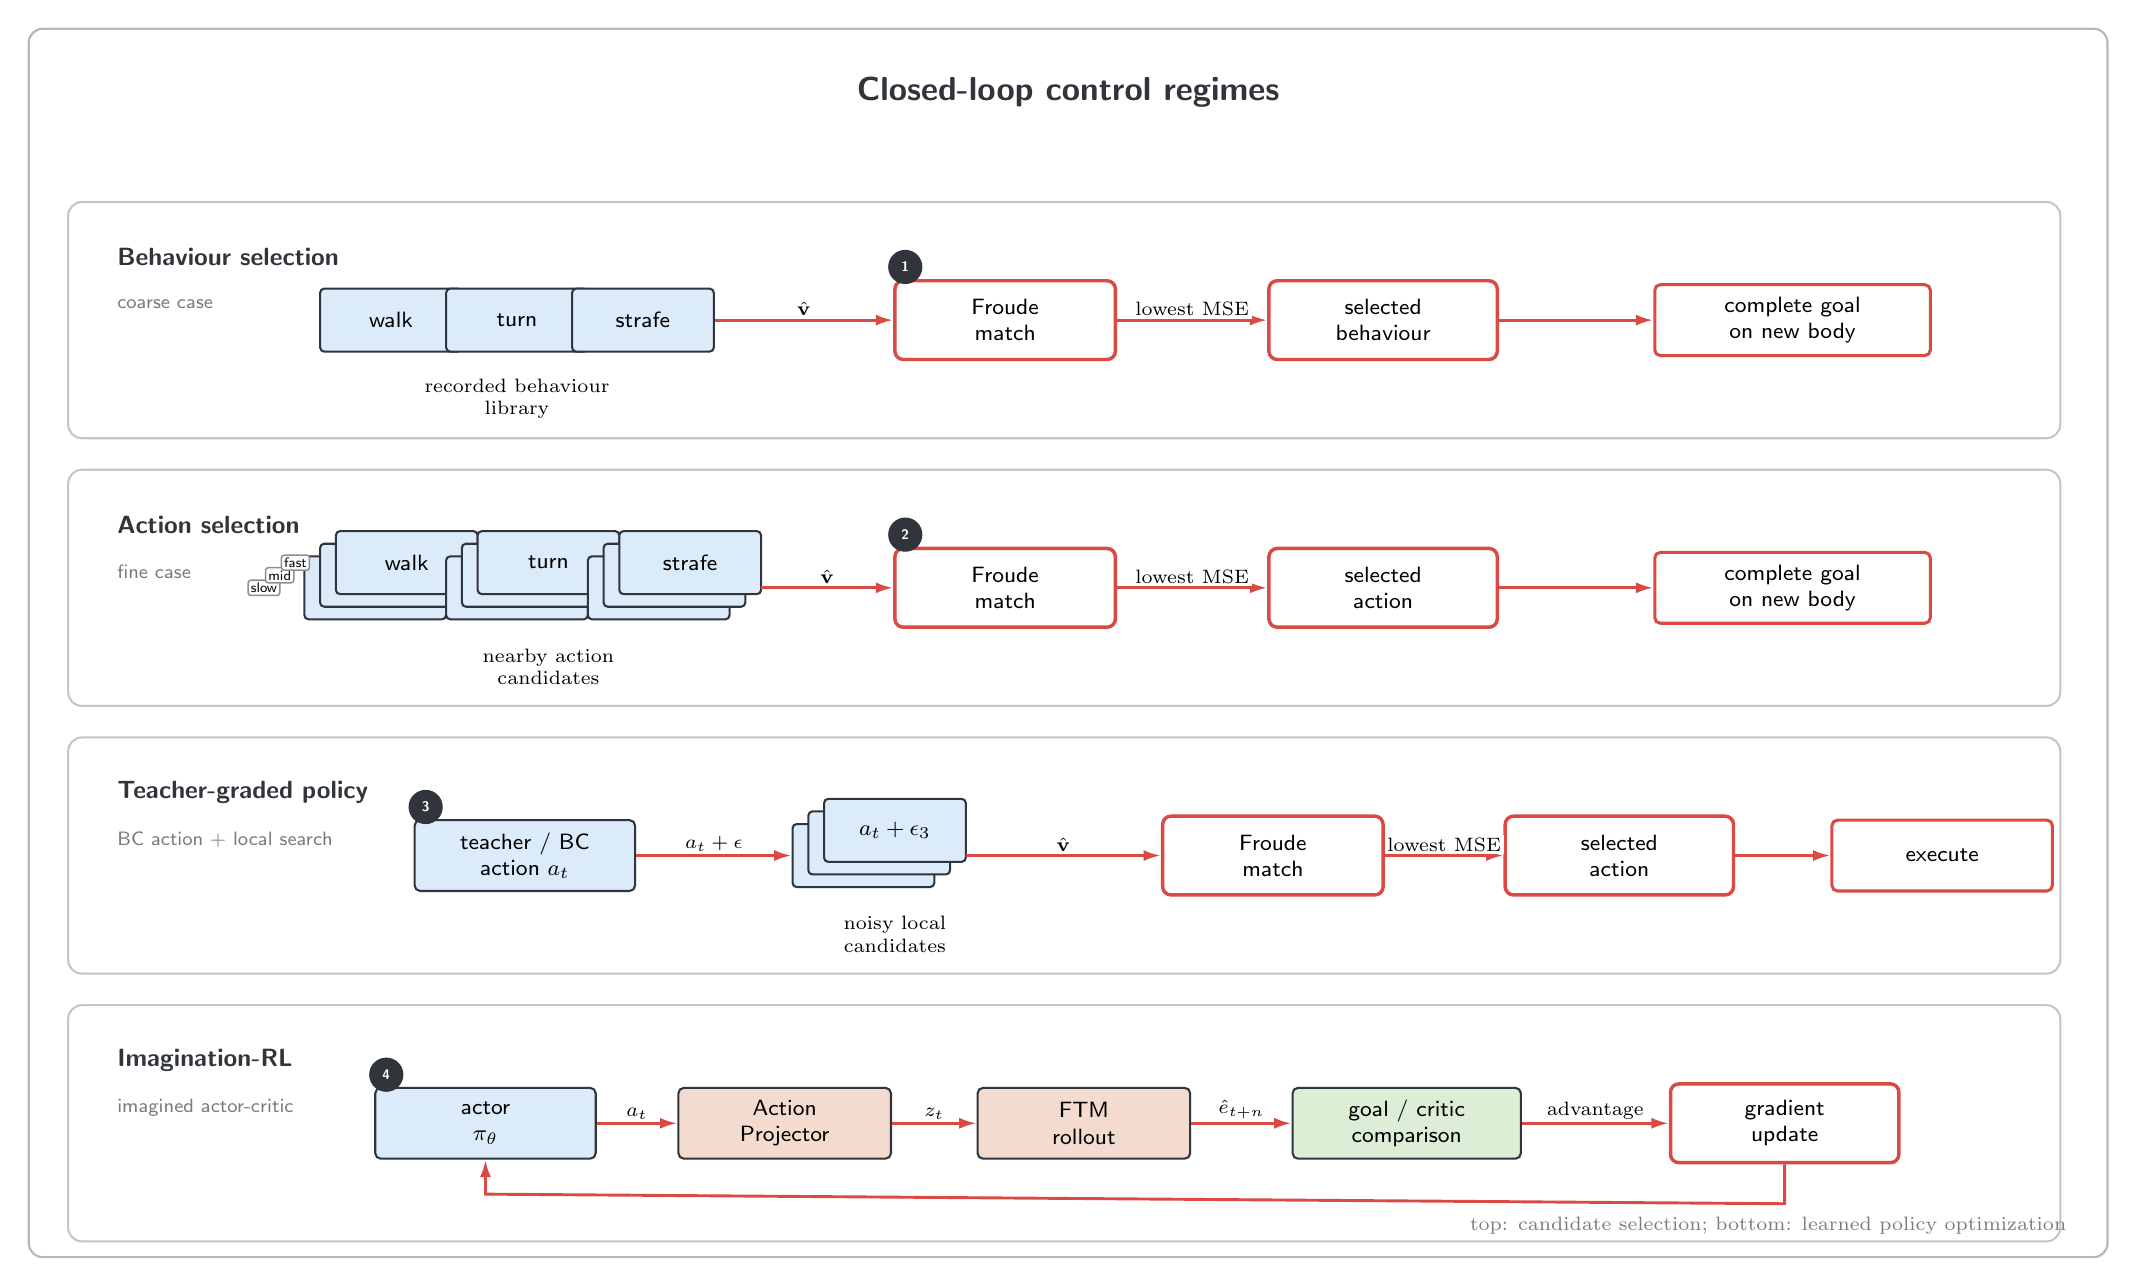
\begin{tikzpicture}[x=1mm,y=1mm]
  \begin{scope}[on background layer]
    \path[draw=ink!35, fill=panel, line width=.8pt, rounded corners=5pt]
      (-8,-80) rectangle (256,76);
  \end{scope}
  \node[font=\sffamily\bfseries\large, text=ink] at (124,68)
    {Closed-loop control regimes};

  % ------------------------------------------------------------------
  % 1. Behaviour selection
  \begin{scope}[shift={(0,39)}]
    \begin{scope}[on background layer]
      \path[card] (-3,-15) rectangle (250,15);
    \end{scope}
    \node[title, anchor=west] at (2,8) {Behaviour selection};
    \node[subtitle, anchor=west] at (2,2) {coarse case};

    \ThreeBoxIcon{behlib}{(54,0)}
    \node[align=center, font=\scriptsize] at (54,-10) {recorded behaviour\\library};
    \node[score] (score1) at (116,0) {Froude\\match};
    \node[selected] (sel1) at (164,0) {selected\\behaviour};
    \node[box, draw=emphasisred, line width=1.1pt, minimum width=35mm] (done1) at (216,0)
      {complete goal\\on new body};

    \draw[hotflow] (behlibc.east) -- node[above,note] {$\hat{\mathbf v}$} (score1.west);
    \draw[hotflow] (score1) -- node[above,note] {lowest MSE} (sel1);
    \draw[hotflow] (sel1) -- (done1);
    \node[steptag, anchor=south west] at (score1.north west) {1};
  \end{scope}

  % ------------------------------------------------------------------
  % 2. Action selection
  \begin{scope}[shift={(0,5)}]
    \begin{scope}[on background layer]
      \path[card] (-3,-15) rectangle (250,15);
    \end{scope}
    \node[title, anchor=west] at (2,8) {Action selection};
    \node[subtitle, anchor=west] at (2,2) {fine case};

    \ThreeActionStackIcon{actlib}{(54,0)}
    \node[align=center, font=\scriptsize] at (58,-10) {nearby action\\candidates};
    \node[score] (score2) at (116,0) {Froude\\match};
    \node[selected] (sel2) at (164,0) {selected\\action};
    \node[box, draw=emphasisred, line width=1.1pt, minimum width=35mm] (done2) at (216,0)
      {complete goal\\on new body};

    \draw[hotflow] (85,0) -- node[above,note] {$\hat{\mathbf v}$} (score2.west);
    \draw[hotflow] (score2) -- node[above,note] {lowest MSE} (sel2);
    \draw[hotflow] (sel2) -- (done2);
    \node[steptag, anchor=south west] at (score2.north west) {2};
  \end{scope}

  % ------------------------------------------------------------------
  % 3. Teacher-graded policy
  \begin{scope}[shift={(0,-29)}]
    \begin{scope}[on background layer]
      \path[card] (-3,-15) rectangle (250,15);
    \end{scope}
    \node[title, anchor=west] at (2,8) {Teacher-graded policy};
    \node[subtitle, anchor=west] at (2,2) {BC action + local search};

    \node[candidate] (teacher) at (55,0) {teacher / BC\\action $a_t$};
    \NoisyStackIcon{noise}{(98,0)}
    \node[align=center, font=\scriptsize] at (102,-10) {noisy local\\candidates};
    \node[score] (score3) at (150,0) {Froude\\match};
    \node[selected] (sel3) at (194,0) {selected\\action};
    \node[box, draw=emphasisred, line width=1.1pt, minimum width=28mm] (done3) at (235,0)
      {execute};

    \draw[hotflow] (teacher) -- node[above,note] {$a_t+\epsilon$} (noisea.west);
    \draw[hotflow] (111,0) -- node[above,note] {$\hat{\mathbf v}$} (score3.west);
    \draw[hotflow] (score3) -- node[above,note] {lowest MSE} (sel3);
    \draw[hotflow] (sel3) -- (done3);
    \node[steptag, anchor=south west] at (teacher.north west) {3};
  \end{scope}

  % ------------------------------------------------------------------
  % 4. Imagination-RL
  \begin{scope}[shift={(0,-63)}]
    \begin{scope}[on background layer]
      \path[card] (-3,-15) rectangle (250,15);
    \end{scope}
    \node[title, anchor=west] at (2,8) {Imagination-RL};
    \node[subtitle, anchor=west] at (2,2) {imagined actor-critic};

    \node[candidate] (actor) at (50,0) {actor\\$\pi_\theta$};
    \node[model] (proj) at (88,0) {Action\\Projector};
    \node[model] (ftm) at (126,0) {FTM\\rollout};
    \node[bodyhead] (critic) at (167,0) {goal / critic\\comparison};
    \node[selected] (update) at (215,0) {gradient\\update};

    \draw[hotflow] (actor) -- node[above,note] {$a_t$} (proj);
    \draw[hotflow] (proj) -- node[above,note] {$z_t$} (ftm);
    \draw[hotflow] (ftm) -- node[above,note] {$\hat e_{t+n}$} (critic);
    \draw[hotflow] (critic) -- node[above,note] {advantage} (update);
    \draw[hotflow] (update.south) -- ++(0,-5) -- (50,-9) -- (actor.south);
    \node[steptag, anchor=south west] at (actor.north west) {4};
  \end{scope}

  \node[font=\scriptsize, text=targetgray, anchor=east] at (252,-76)
    {top: candidate selection; bottom: learned policy optimization};
\end{tikzpicture}%
}
\vspace*{\fill}
\end{document}
